%!TEX root = ../TTT4150-Summary.tex
\section{Spherical geometry}

\begin{figure}[htbp]
	\centering
	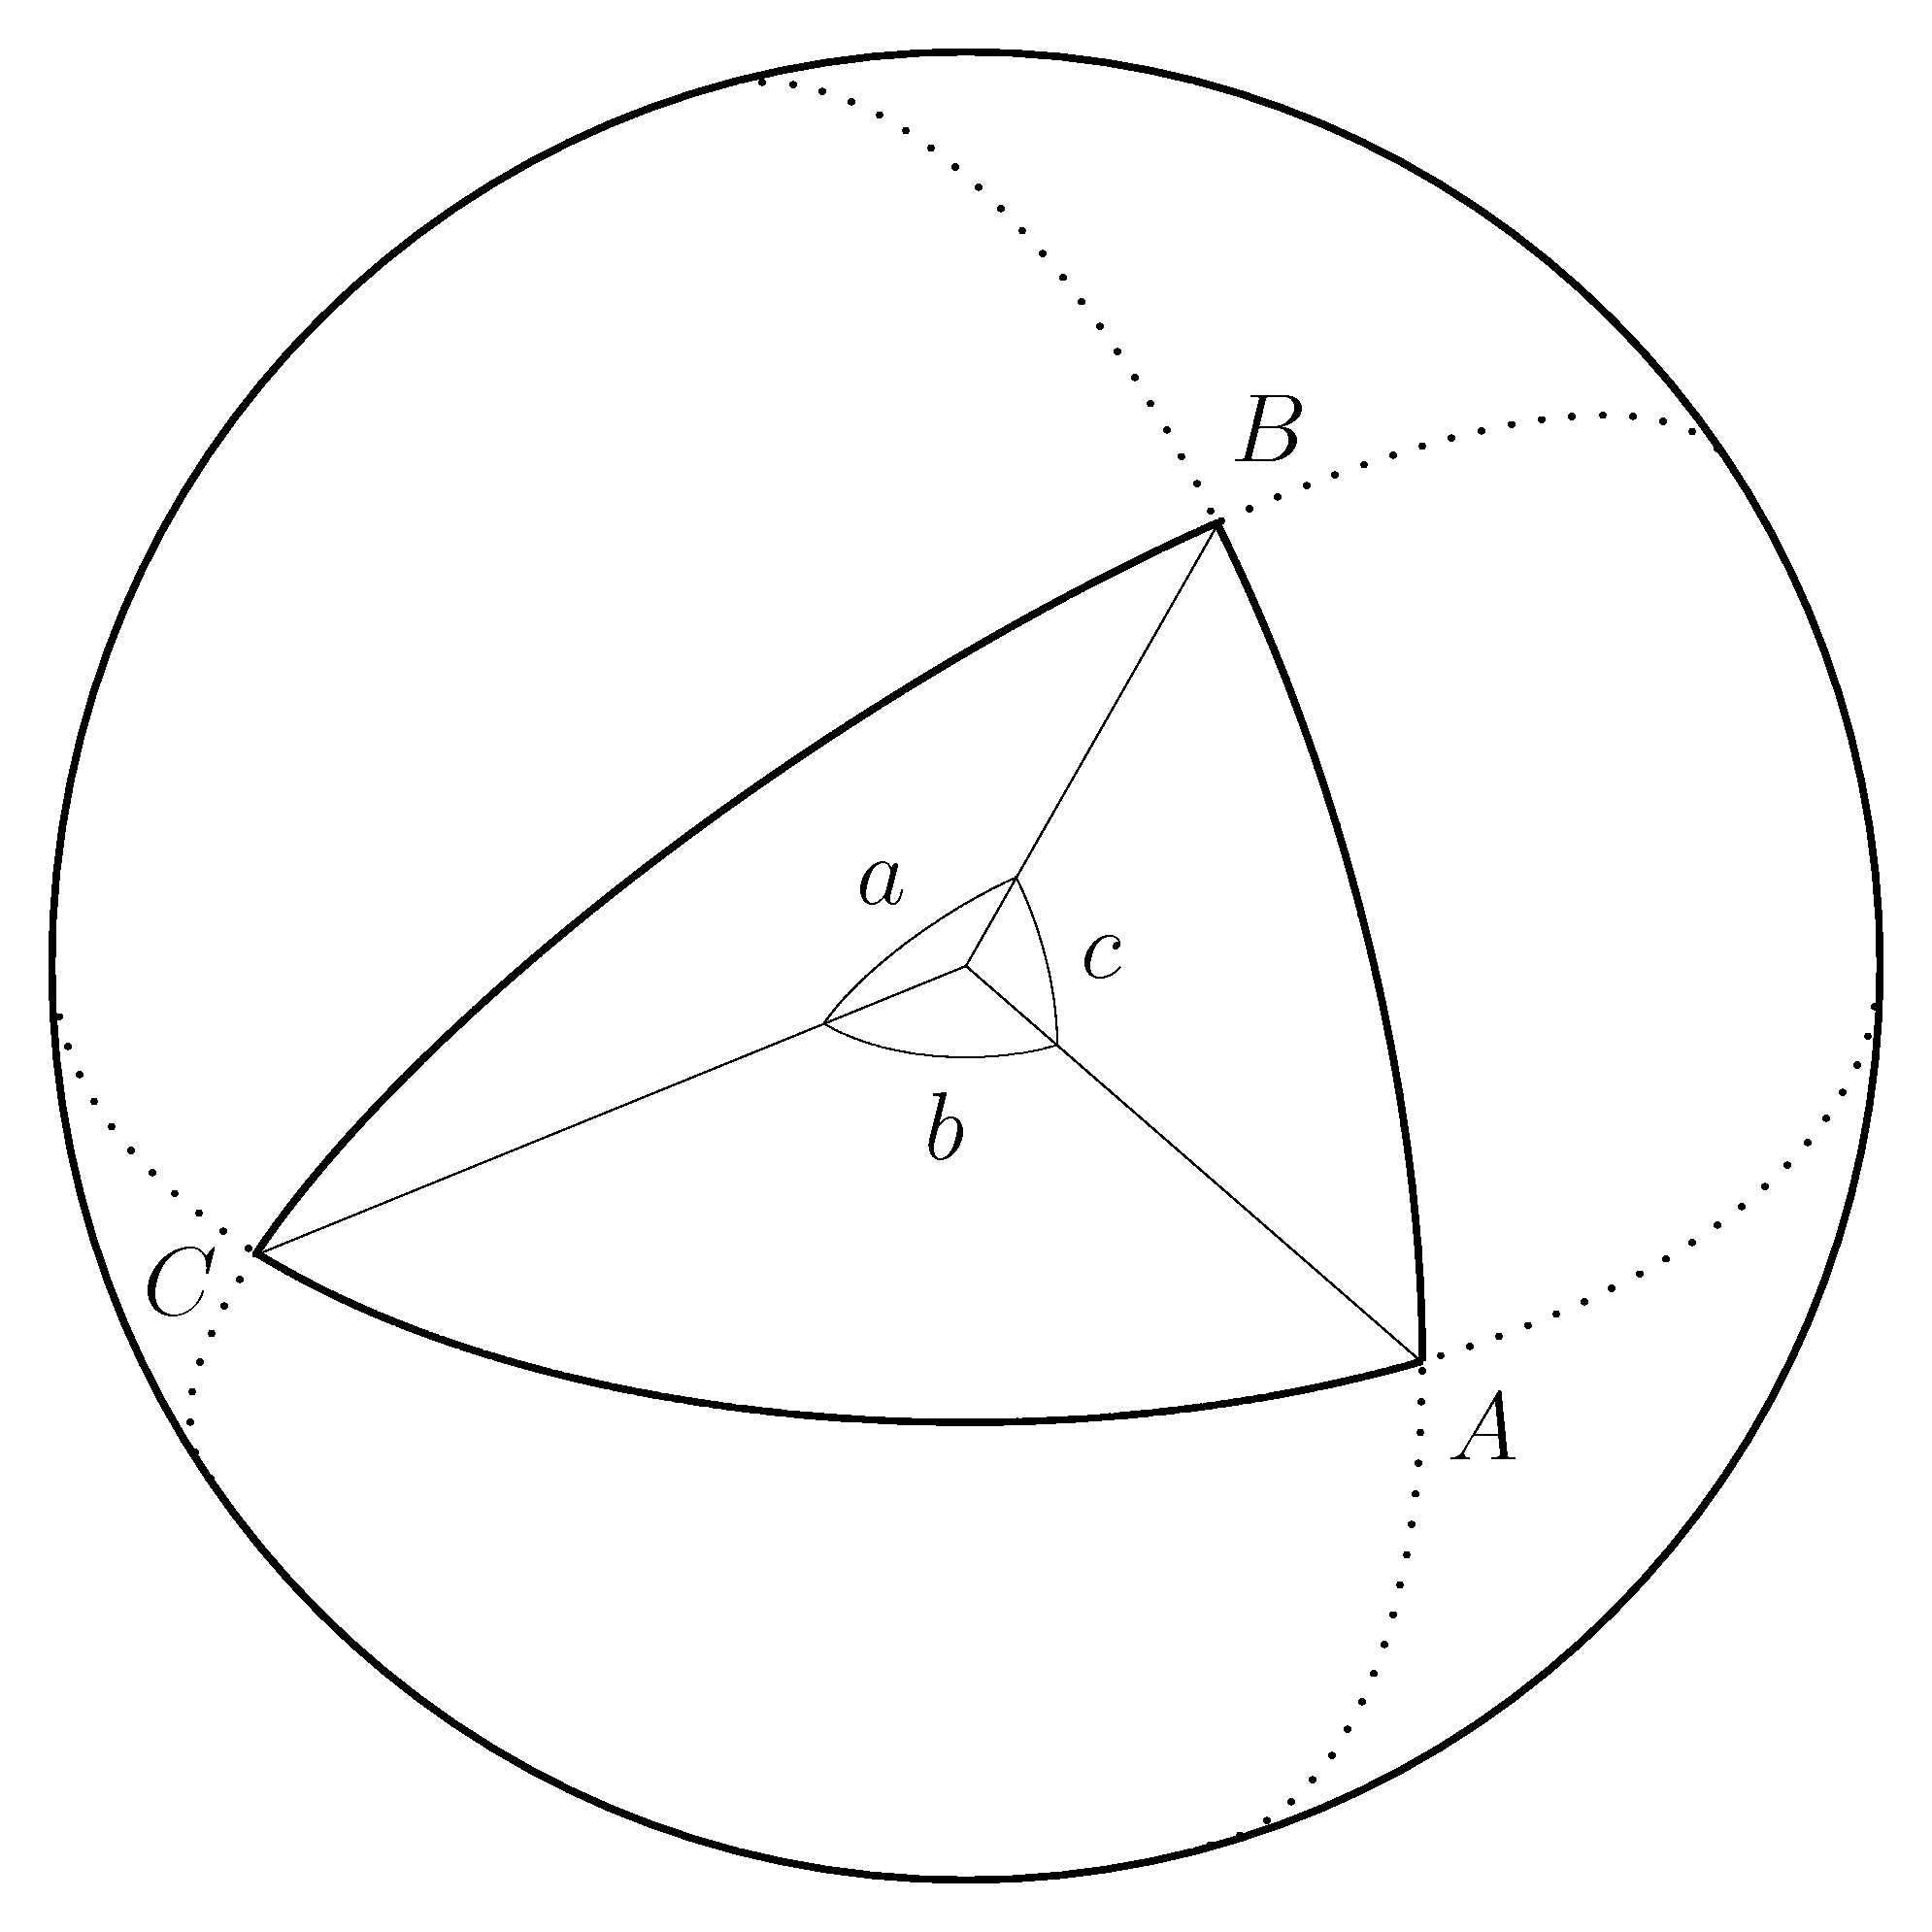
\includegraphics[width=.6\linewidth]{img/spherical_triangle}
	\caption{A triangle on a sphere}
	\label{fig:spherical-triangle}
\end{figure}
A triangle on a sphere is defined by three points on the sphere, as in Figure \ref{fig:spherical-triangle}. Each corner $A$, $B$, and $C$ has an angle, and each line/arc segment has an angle $a$, $b$, and $c$.

Modified cosine rules
\begin{equation}
\begin{split}
	\cos a &= \cos b \cdot \cos c + \sin b \cdot \sin c \cdot \cos A \\
	\cos b &= \cos c \cdot \cos a + \sin c \cdot \sin a \cdot \cos B \\
	\cos c &= \cos a \cdot \cos b + \sin a \cdot \sin b \cdot \cos C
\end{split}
\end{equation}
and sine rules
\begin{equation}
	\frac{\sin A}{\sin a} = \frac{\sin B}{\sin b} = \frac{\sin C}{\sin c}
\end{equation}
apply.

%%%%%%%%%%%%%%%%%%%%%%%%%%%%%%%%%%%%%%%%%%%%%%%%%%%%%%%%%%%%
\subsection{Intersection between great circles}

Each great circle is defined by two points on the surface of a sphere.
\begin{enumerate}
	\item Convert the points to cartesian coordinates.
	\item blabla
\end{enumerate}
